
\chapter{実装}
\label{chap:implementation}

本章では、前章で提案した生活の簡素化支援システムの実装に関する要件と設計について述べる。

\newpage

\section{機能}
本システムでは、部屋内のモノをARで再現し、仮想的に代替することで、本来利用している部屋と同程度の環境の再現を行う。どのような部屋に対しても同様の環境を作ることができる事を条件とし、マーカーに対してモノを表示する、画像認識型ARを採用した。部屋内に配置されたマーカーを認識することにより、その位置を中心として、対応する3Dないし2Dのモノを表示する。部屋にマーカーを貼るだけで環境の準備ができ、表示位置の再設定や、他所への持ち運びなども容易である。

\section{基本構成}

本システムのデバイスには、Microsoft社の提供するHololensを使用している。スタンドアロンで動作するARグラスであり、着用したままであっても、日常を過ごす事ができる。Hololens上で動作するソフトウェアの実装には、Unity\cite{unity}, vuforia\cite{vuforia}を使用した。予めマーカー画像を準備した部屋内でHololensを装着し、本システムを起動することで動作する。

マーカーには、processingで生成したランダムな画像を使用した。

\begin{figure}[htbp]
  \begin{minipage}{0.5\hsize}
    \begin{center}
      \fbox{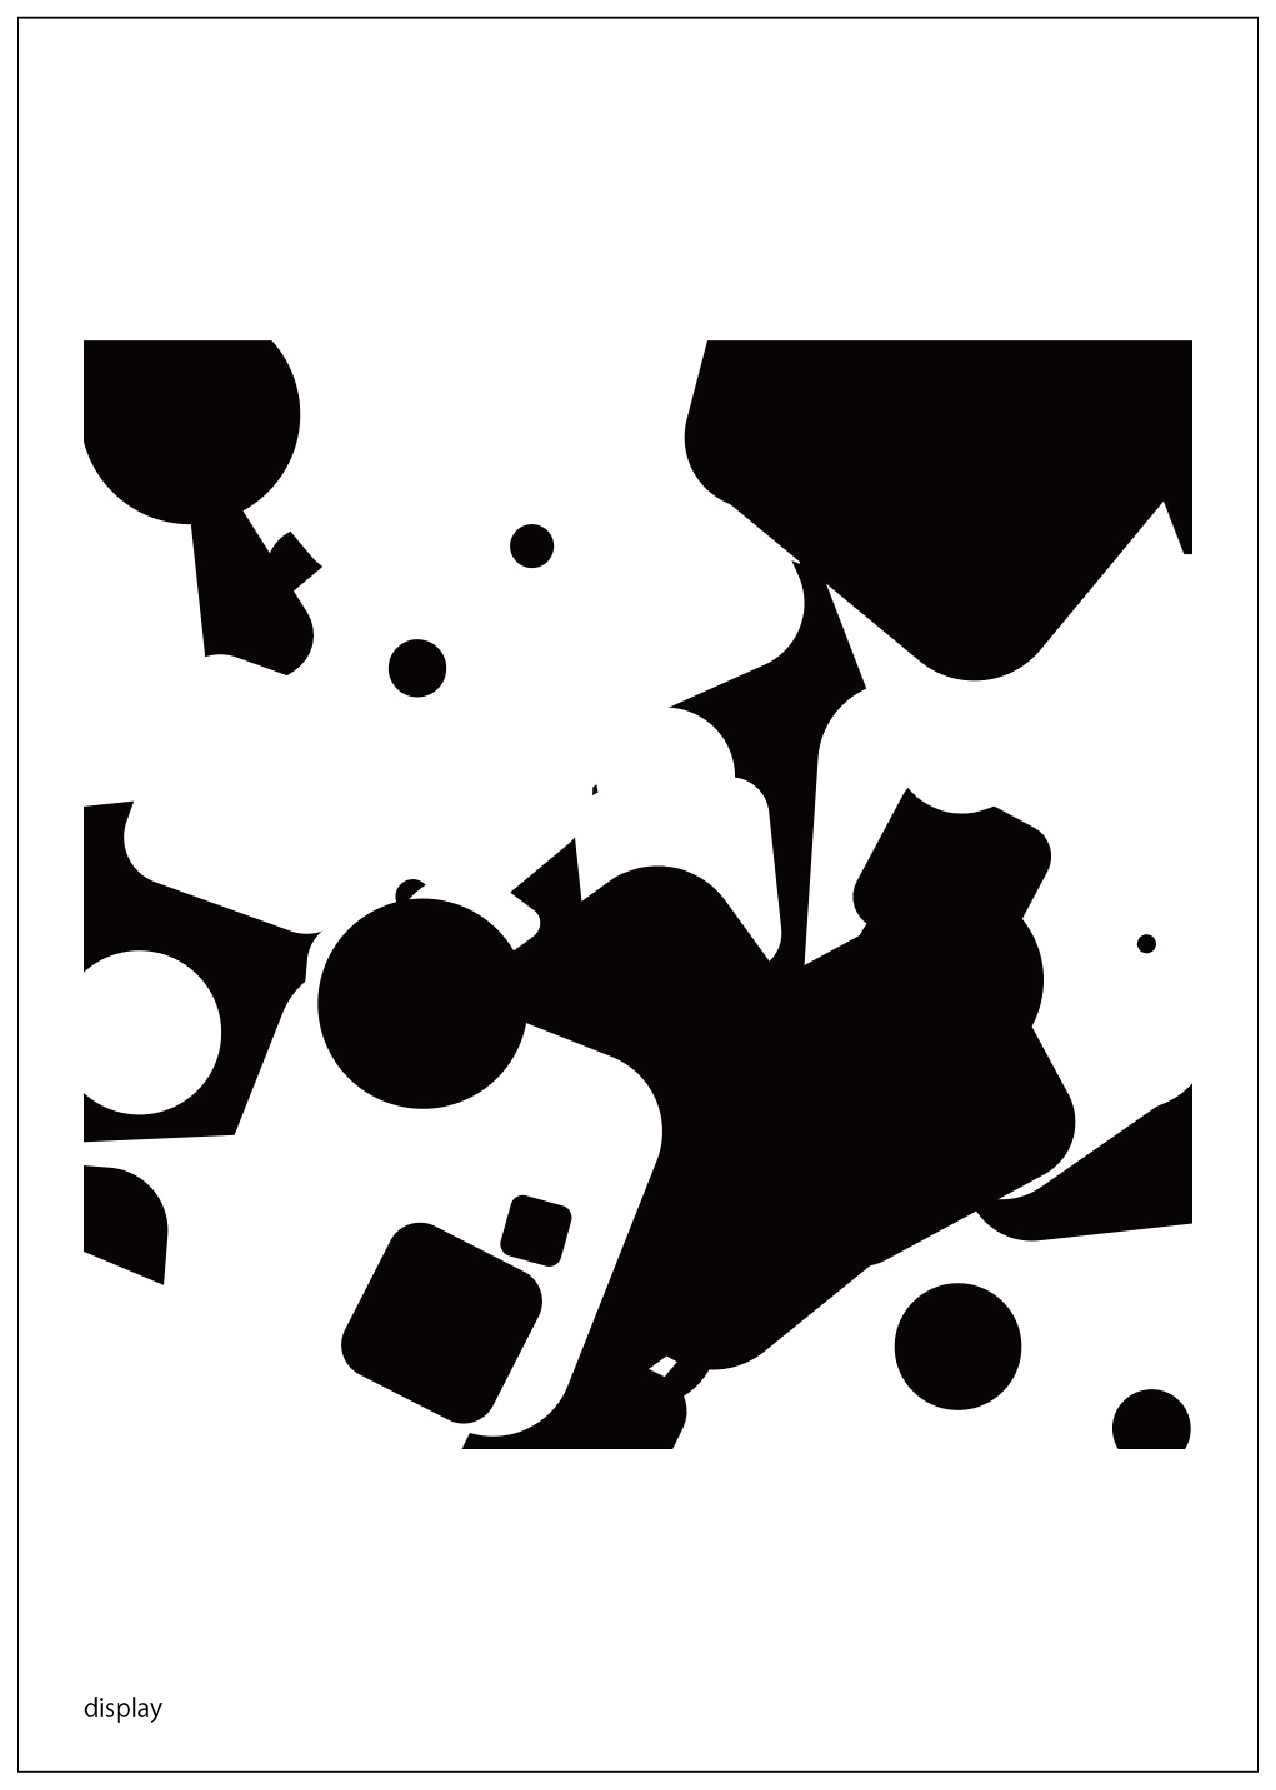
\includegraphics[width=60mm]{images/marker.png}}
    \end{center}
    \caption{使用したマーカー}
  \end{minipage}
  \begin{minipage}{0.5\hsize}
    \begin{center}
      \fbox{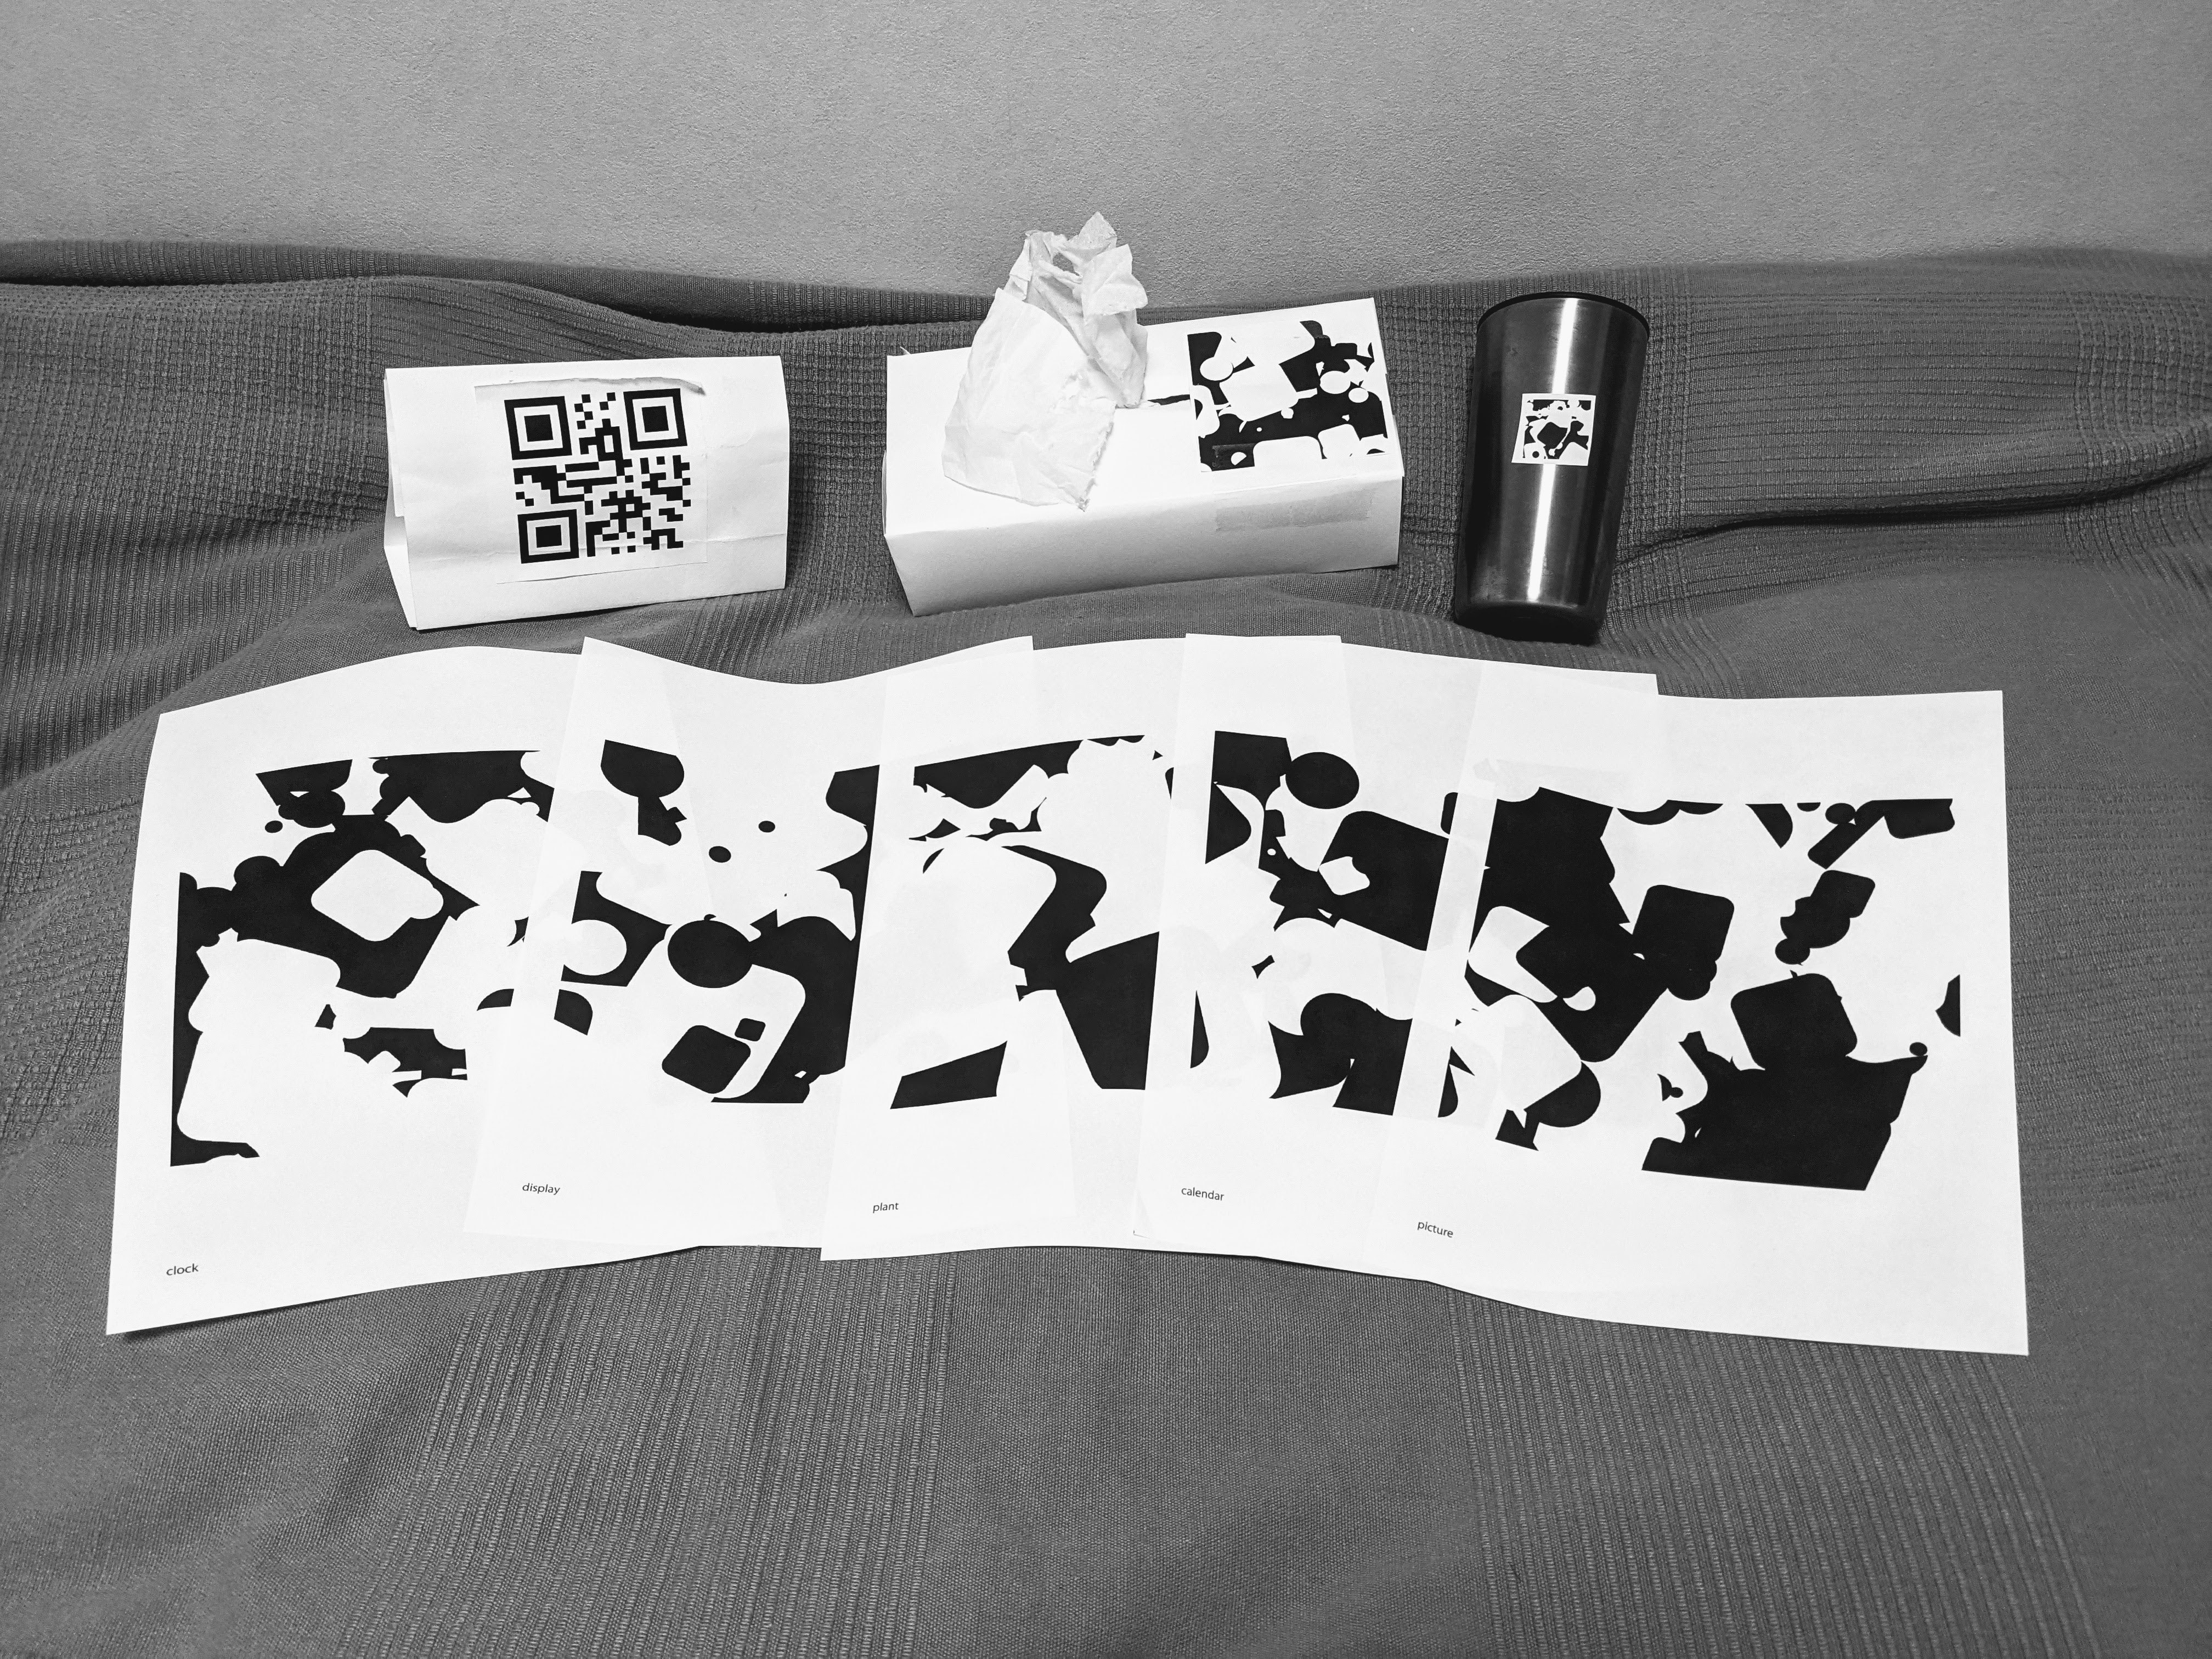
\includegraphics[width=60mm]{images/markers.jpg}}
    \end{center}
    \caption{部屋に置いたマーカー}
  \end{minipage}
\end{figure}


\section{実装}

\subsection{準備}

本提案の要件を最大限に反映するため、空き部屋となっているアパートの一室にてシステムを運用した。システム運用時には、物を置くための机一つを持ち込み、その他は、アパートに備え付けられたもののみがある状態とした。

本システムでは、絵画、カレンダー、壁掛け時計、ディスプレイ、植物、ティッシュの外箱、タンブラー、デジタル時計の合計8つのサンプルコンテンツを用意した。

絵画、カレンダー、壁掛け時計、ディスプレイに対応する四つのマーカーは、一般的な配置場所通り、壁に配置した。また、植物に対応したマーカーは、ARで代替されたの観賞用インテリアの新たな試みとして、壁に配置した。

ティッシュの外箱は、白の用紙で覆ってパッケージが見えない状態にし、マーカー画像を貼り付けた。デジタル時計は、時計そのものではなく、折って三角柱状にした物にマーカーを貼り付けた。ARグラスを通して確認することで、デジタル時計が表示され、その機能を果たす形式となっている。タンブラーには、内容物に対応したパッケージが表示されるマーカーを貼った。

\begin{figure}[htbp]
  \begin{center}
     \fbox{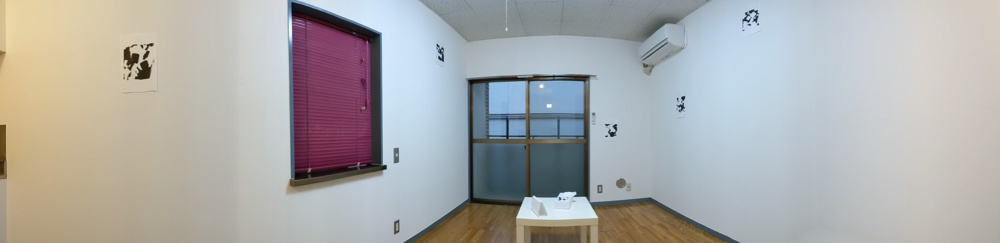
\includegraphics[width=100mm]{images/room_panorama.jpg}}
  \end{center}
  \caption{システムを運用した部屋のパノラマ}
  \label{fig:sample1}
\end{figure}

\subsection{システムの運用}

Hololensを装着し、本システムを起動する事で、hololensに付いているカメラの映像の画像認識が開始される。マーカーを注視する事で、対象のマーカーが認識され、そこに対象のコンテンツが表示される。コンテンツはマーカーに追従するため、マーカーの付いている物体を移動しても問題はない。

\begin{figure}[htbp]
  \begin{minipage}{0.5\hsize}
    \begin{center}
      \fbox{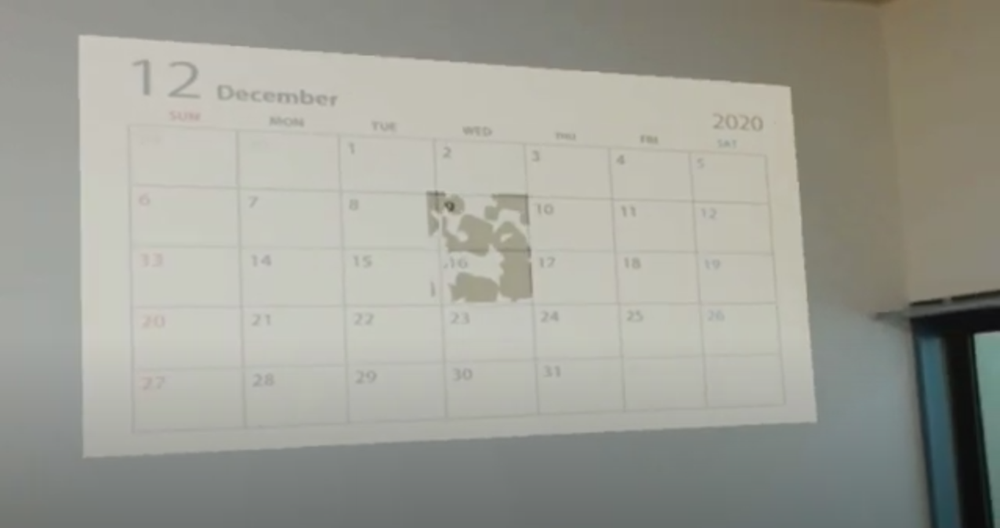
\includegraphics[width=60mm]{images/test_calendar.png}}
    \end{center}
    \caption{仮想的に代替したカレンダー}
  \end{minipage}
  \begin{minipage}{0.5\hsize}
    \begin{center}
      \fbox{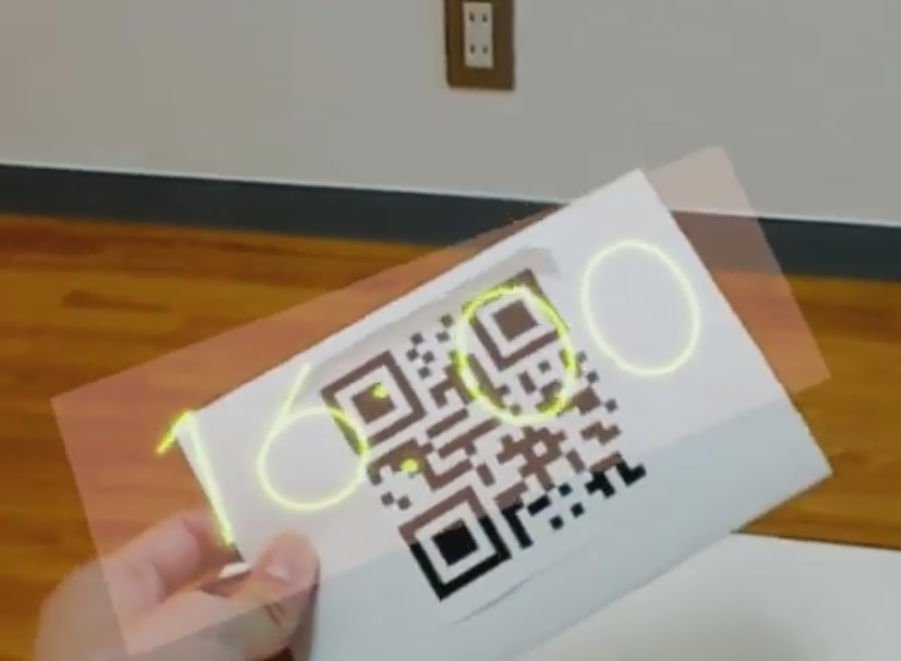
\includegraphics[width=60mm]{images/test_digital_clock.png}}
    \end{center}
    \caption{仮想的に代替したデジタル時計}
  \end{minipage}
\end{figure}

